\section{Parameterization of the magnet kick}
\label{sec:kick}
 %
As will be discussed in Section \ref{sec:ep} to model the momentum
resolution it is beneficial to use information on the track position after the magnet. \textbf{RapidSim}
has in place a single kick parameterization based upon the publicly
available studies described in
Ref.~\cite{VanTilburg:691686}. Based upon eye-balling this plot and taking
reasonable values for the track slopes before and after the magnet in
\textbf{RapidSim} a kick of $1.2 \gevc$ is applied at $z = 5.4 ~\textrm{m}$.  Since the referenced work
is rather old and the procedure to determine the kick parameters
rather coarse it was decided to redo this study. This leads to an
improved parameterization for use in \textbf{RapidSim}.

The magnet field parameterization is made using the  $\chicone \rightarrow J/\psi \mu^+ \mu^-$ and $\Upsilon(1S) \rightarrow
\mu^+ \mu^-$ simulation samples, selecting tracks from truth matched
candidates. To determine the effective magnetic
centre where the kick takes place the track state before and after the
magnet is needed. The track parameters before the magnet are easily
available from a \textbf{DecayTreeTuple}. A tool exists \footnote{TupleToolTrackPosition} to give
 the track position at given $z$. Storing the track $x$ and $y$ at $z
 = 9.2~\textrm{m} $ and $z
 = 10~\textrm{m}$ allows the track state after the magnet in a field
 free region to be estimated. From these two lines the intersection
 point at the magnet centre is easily calculated. This procedure is
 relatively crude but as will be seen gives a precision sufficient
 for these studies \footnote{It would be better to us MC truth both
   before and after the magnet. However, the latter information is not
 stored on the DST.}. Fig.~\ref{fig:zc} shows the
 distribution of the calculated magnet centre. The mode of this
 distribution ($z_c = 5.26 \textrm{m}$) is taken as the magnet centre
 \footnote{It is known that $z_c$ depends on the tracks kinematics but
   for the accuracy needed here a single value is
   considered sufficient. }.
\begin{figure}[htb!]
\begin{center}
\resizebox{4.0in}{!}{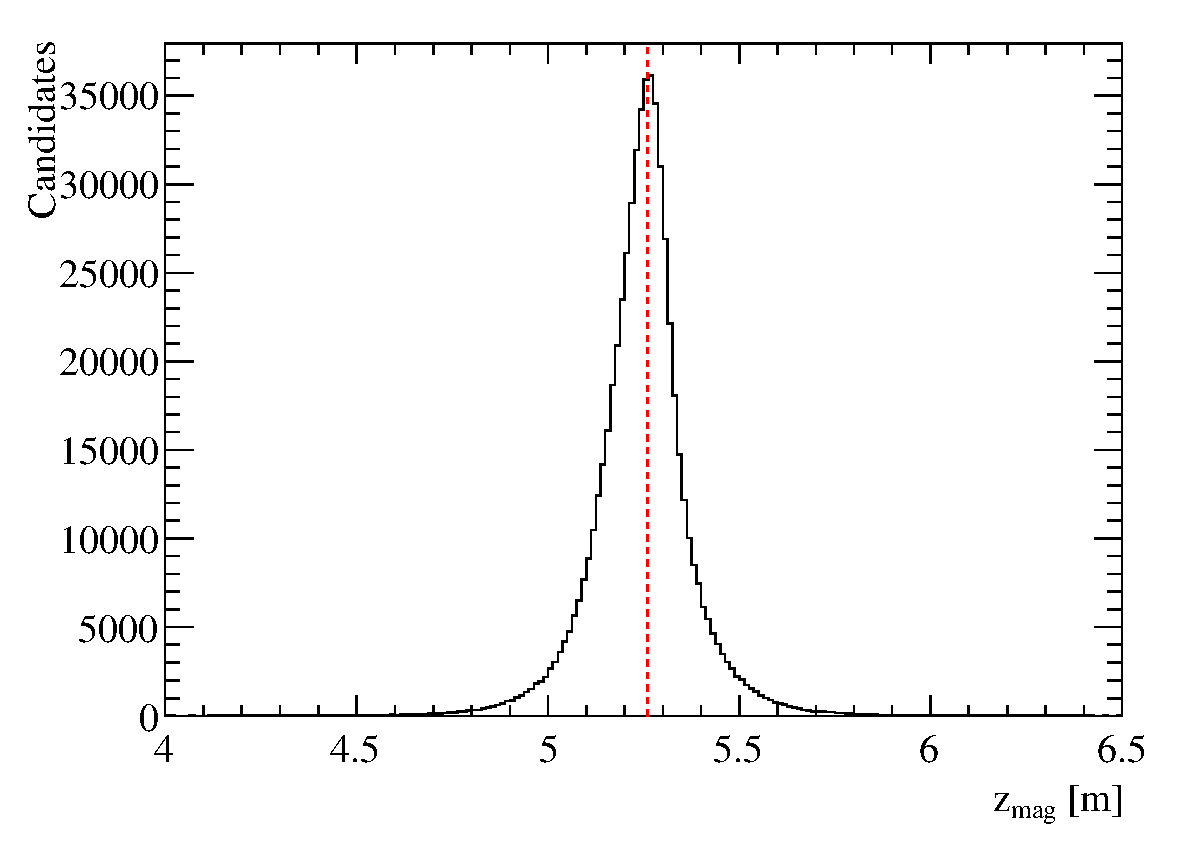
\includegraphics{figs/zc.pdf}}
\caption{\small Distribution of the estimated magnet centre calculated
  using tracks from the $\chicone$ and $\Upsilon$ samples. The
  dotted red line shows the mode of the distribution $z_c = 5.26~\textrm{m}$. }
\label{fig:zc}
\end{center}
\end{figure}

From the studies in  Ref.~\cite{VanTilburg:691686} is it known the
size of the kick of the magnet increases with $ty$. This can be seen
in Fig.~\ref{fig:by} where the $\pt$ kick of the magnet is plotted
versus $ty$. As in the previous study is found that this shape can be
modelled with a second-order polynomial.
\begin{figure}[htb!]
\begin{center}
\resizebox{4.0in}{!}{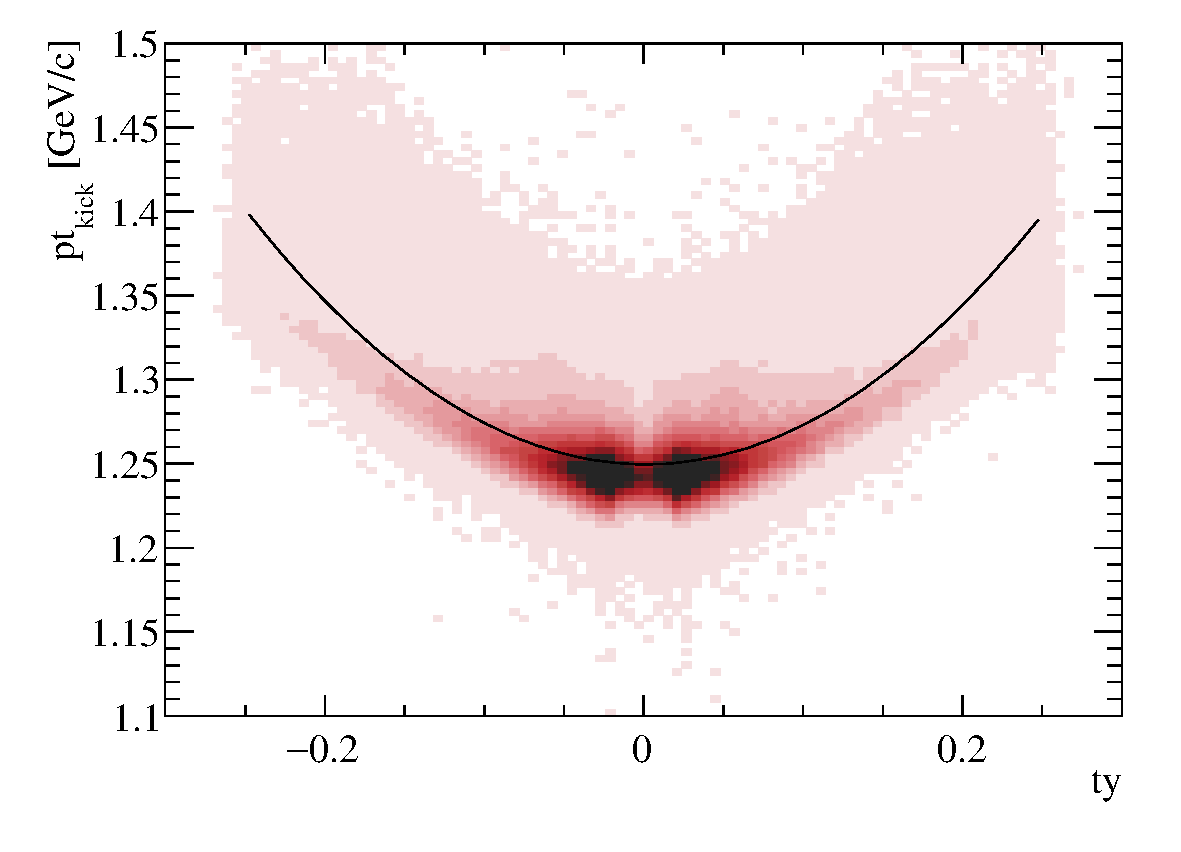
\includegraphics{figs/by.pdf}}
\caption{\small $\pt$ kick versus $ty$. A fit to a second order
  polynomial is superimposed. The coefficients of the polynomial are $1.25
  \gevc$, $-0.006~\gevc$ and $2.45~\gevc$. }
\label{fig:by}
\end{center}
\end{figure}

Fig.~\ref{fig:dx} shows the difference between the x-position
calculated by the track fit at $z = 9.2~\textrm{m}$ and the single-kick
parameterization above. The RMS of the distribution is $0.8 ~\textrm{cm}$
which is adequate for our needs. Performing the same exercise
in $y$ (where the only effect is multiple scattering) gives a precision of $0.5~\textrm{cm}$. This means that
the precision of the parameterization is around $0.6 \textrm{cm}$. 

An interesting question is the gain in precision compared to the
parameterization currently used in \textbf{RapidSim}. Using that the
RMS of the distribution is broadened to $1.5~\textrm{cm}$ and there is
a clear double peak structure reflecting the fact the parameterization
leads a to a bias of $1~\textrm{cm}$ for each charge (Fig.\ref{fig:dxsimple}). Clearly the new
parameterization is better though all things considered the old
parameterization was not so bad.
%
\begin{figure}[htb!]
\begin{center}
\resizebox{4.0in}{!}{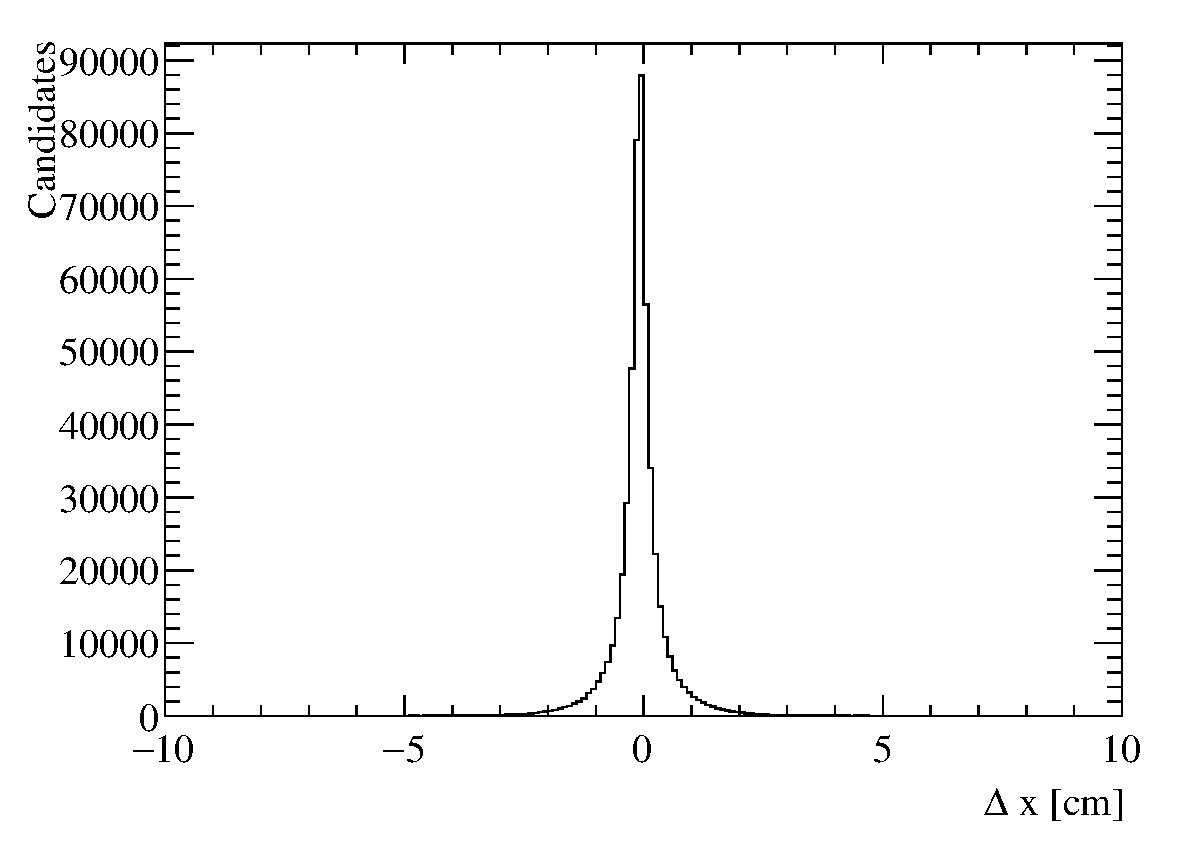
\includegraphics{figs/dx.pdf}}
\caption{\small Difference between the x-position
calculated by the track fit at $z = 9.2~\textrm{m}$ and the single-kick
parameterization.}
\label{fig:dx}
\end{center}
\end{figure}
%
\begin{figure}[htb!]
\begin{center}
\resizebox{4.0in}{!}{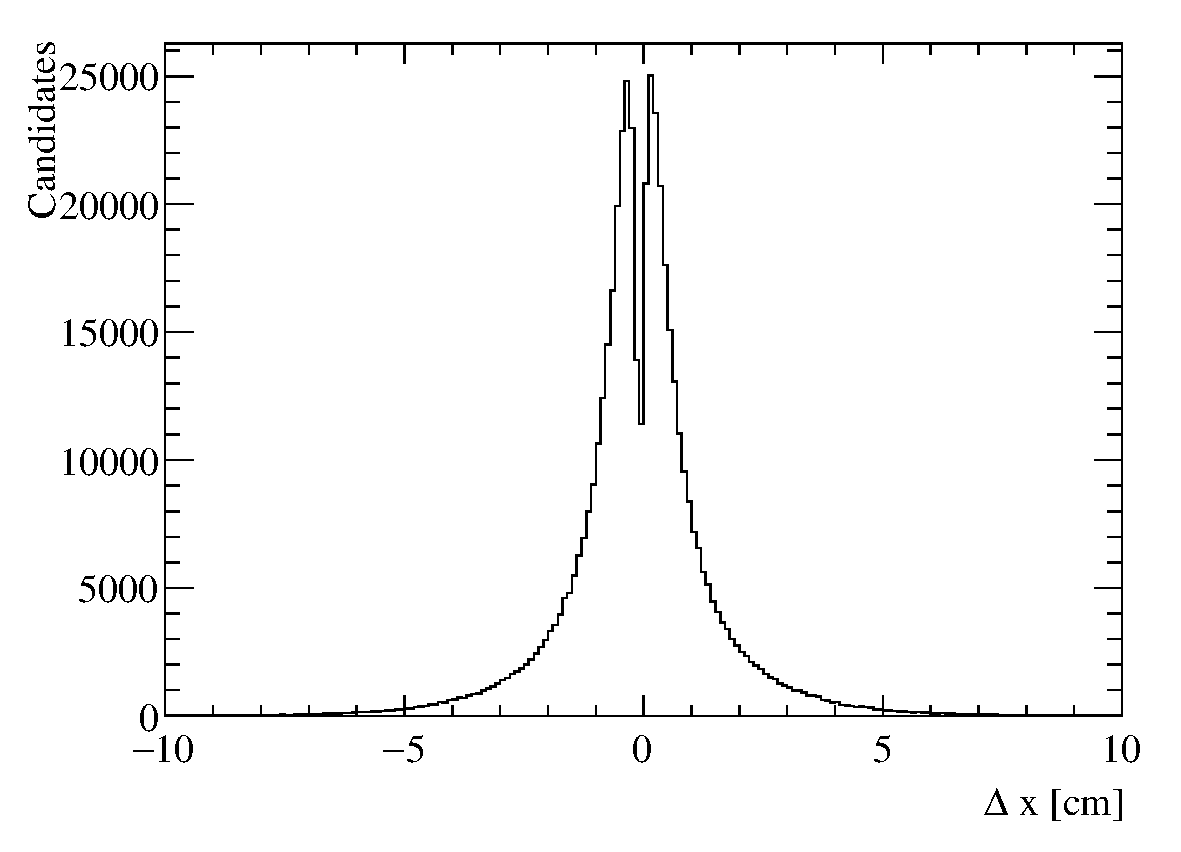
\includegraphics{figs/simple.pdf}}
\caption{\small Difference between the x-position
calculated by the track fit at $z = 9.2~\textrm{m}$ and the default single-kick
parameterization in \textbf{RapidSim}.}
\label{fig:dxsimple}
\end{center}
\end{figure}
%